\section{Building Generation}

\begin{figure}[H]
  \centering

  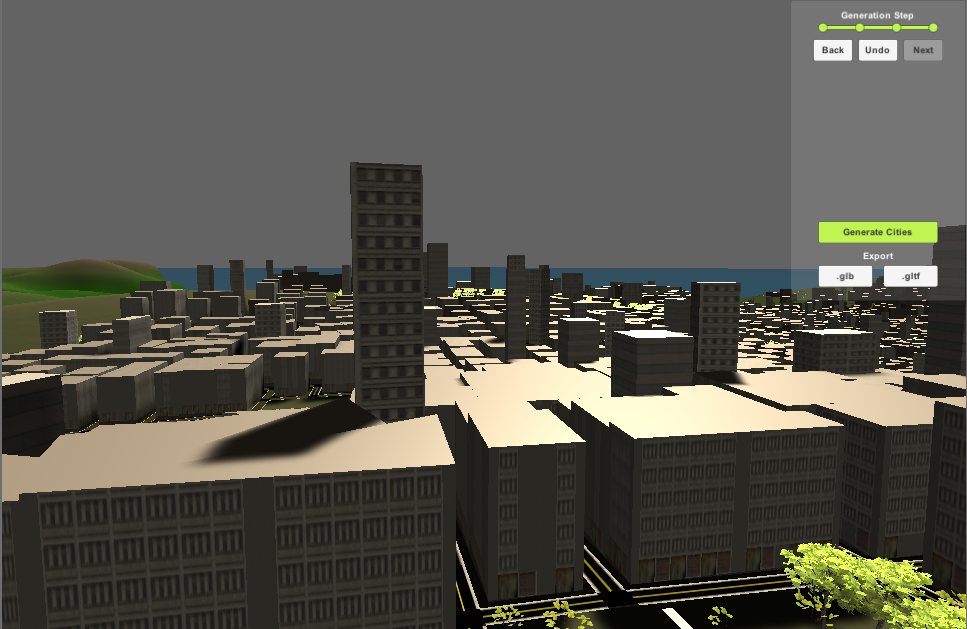
\includegraphics[width=0.7\textwidth]{figure/skyline.PNG}
  \caption{Skyline of \textit{Manhattan} and \textit{Skyscraper} buildings together.}

  \label{fig:skyline-result}
\end{figure}


The Building Generator creates buildings for the plots whose labels are \textit{Manhattan} or \textit{Skyscraper}. 
An example of a skyline with both \textit{Manhattan} and \textit{Skyscraper} can be seen in Figure \ref{fig:skyline-result}.
\textit{Manhattan} buildings are very versatile via the possibility to have different floor types L-systems and different wall segment L-systems.
The final implementation had one floor type generator and four wall segment generator. 
The floor type generator always generated the first floor with \textit{FirstFloor} type.
After that, it repeats one of three remaining floor types until the desired height has been met. 
Note first that each wall segment generation starts and ends with a corner segment. 
Explanation of the four floor types, and its wall segment generation:

\begin{itemize}
  \item \textit{FirstFloor} - generates a combination of shop windows, walls, and doors. 
  \item \textit{NormalFloor} - generates wall and window segments, but it only generates half of the wall. For the other half, it copies the first half and reverses it. 
  \item \textit{EveryOtherFloor} - alternates between wall and window segments.
  \item \textit{RepeatWindowFloor} - only generates window segments.
\end{itemize}

In Figure \ref{fig:wall-segment-generator}, there are examples of the one floor type generator and the four different wall segment generators.

\begin{figure}[H]
  \centering

  \begin{subfigure}[b]{0.25\textwidth}
    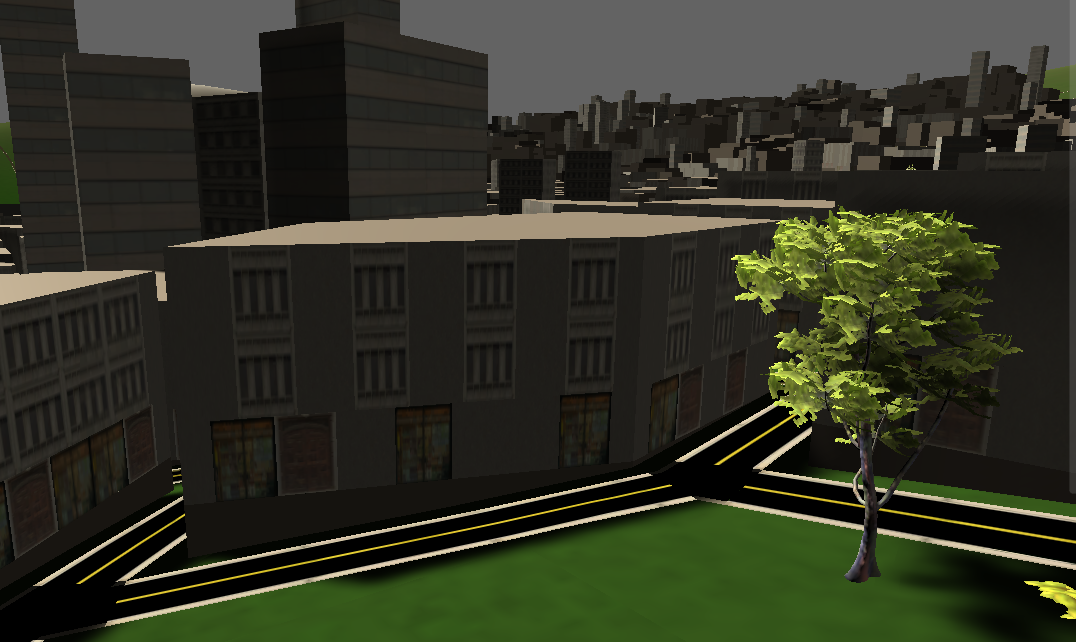
\includegraphics[width=\textwidth]{figure/building-every-other.PNG}
    \caption{\textit{EveryOtherFloor}.}
  \end{subfigure}
  \quad
  \begin{subfigure}[b]{0.25\textwidth}
    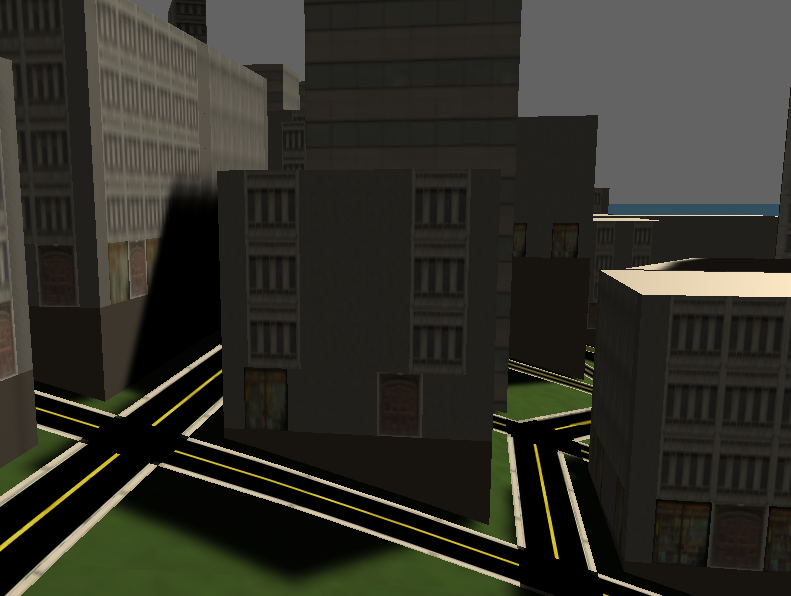
\includegraphics[width=\textwidth]{figure/building-normal.PNG}
    \caption{\textit{NormalFloor}.}
  \end{subfigure}
  \quad
  \begin{subfigure}[b]{0.25\textwidth}
      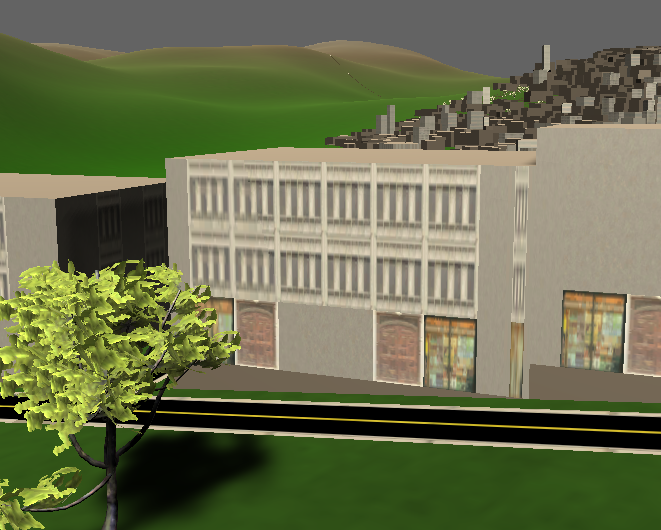
\includegraphics[width=\textwidth]{figure/building-only-window.PNG}
      \caption{\textit{RepeatWindowFloor}.}
  \end{subfigure}
  
  \caption{The three different wall segment generators. Notice that each building has a \textit{FirstFloor} wall segment generator on the first floor.}
  \label{fig:wall-segment-generator}
\end{figure}

Skyscraper has two different textures from which different sub-regions were sampled. In Figure \ref{fig:skyscraper-result}, you can see examples of them. 

  \begin{figure}[H]
    \centering
  
    \begin{subfigure}[b]{0.45\textwidth}
      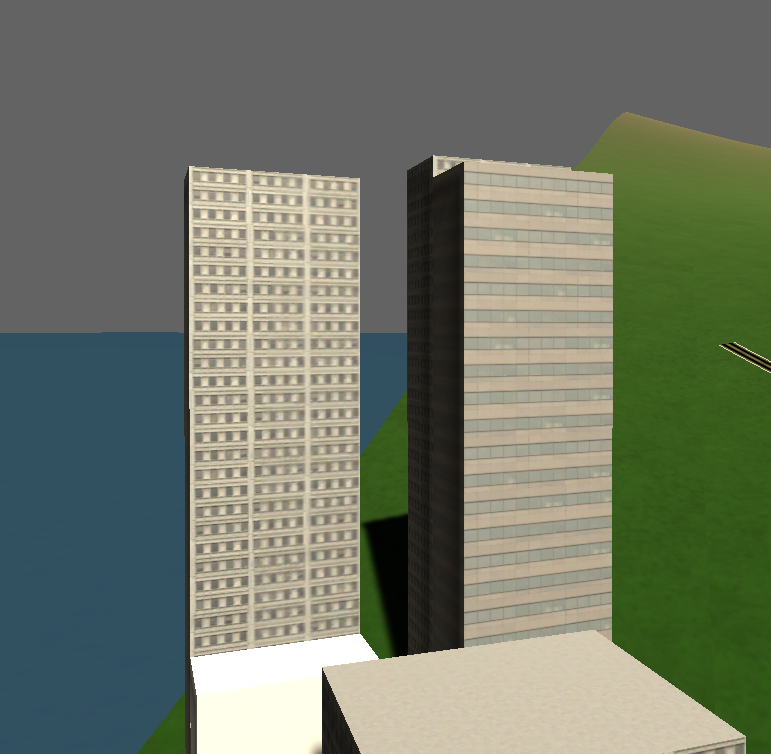
\includegraphics[width=\textwidth]{figure/skyscraper-close-up.PNG}
    \end{subfigure}
    \quad
    \begin{subfigure}[b]{0.45\textwidth}
      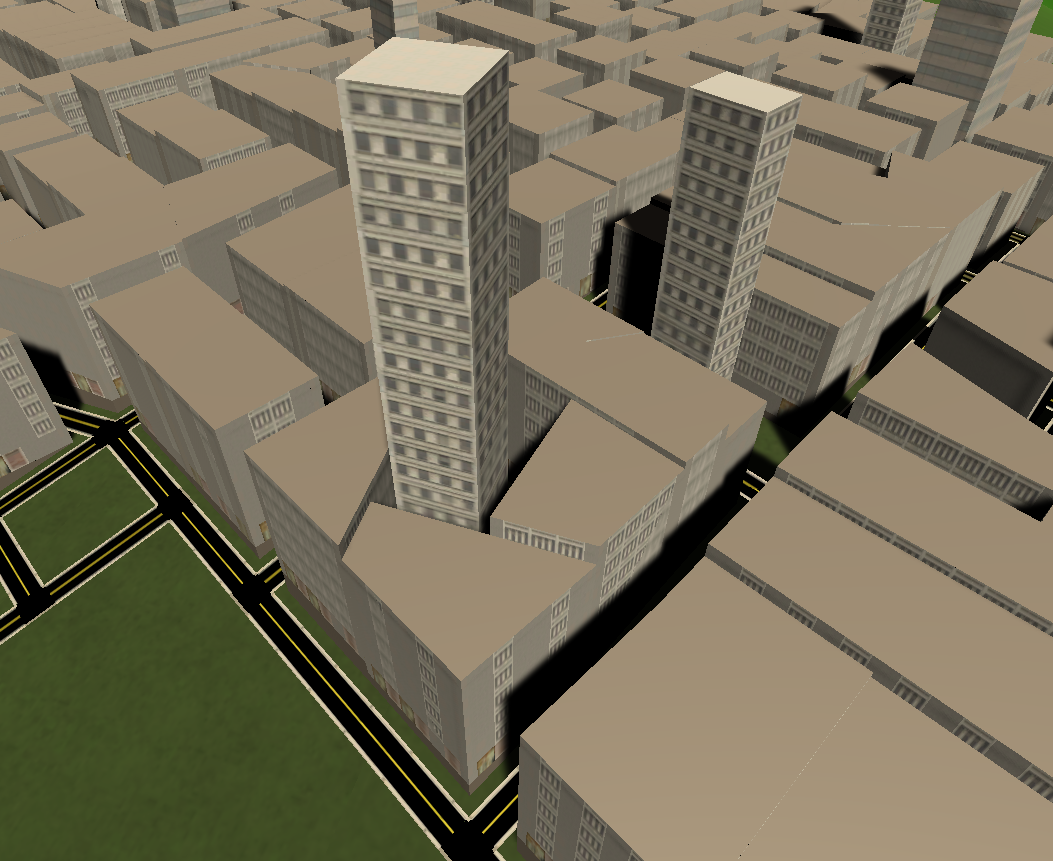
\includegraphics[width=\textwidth]{figure/wack.PNG}
    \end{subfigure}
    
    \caption{Various \texit{Skyscraper}s.}
    \label{fig:skyscraper-result}
  \end{figure}
 